\section {Co-designed Ising Machine Architecture}
\label{sec:arch}


%In this section, we discuss about the algorithm change to QUBO formulation of decoding of LDPC codes and it's formulation.
\subsection{Fundamentals of QUBO formulation of LDPC decoding}
\label{sec:QUBO_formulation}

The goal of LDPC decoding is to reproduce the original message $M$ with low bit error rates. 
This is modeled as a combinatorial optimization problem with two objectives: \begin{enumerate}
    \item The decoded output $\tilde{C}$ is a code word (satisfies parity check).
    \item It should be close to the received message $R$.
\end{enumerate}
If we use the BPSK modulation scheme, the objective function can be represented by Eq.~\ref{eq::obj}
where $\alpha$ adjusts the relative emphasis of the two objectives above.\footnote{Choosing $\alpha > \sum_{i=1}^{n} 4|R_i|$ is suggested~\cite{tawada2020new} to \emph{guarantee} the decode output is always a code word. In our observations, this choice results in poorer results than using empirically selected values.} \begin{equation}
\label{eq::obj}
\begin{split}
    F =  \sum_{i=0}^{n-1}(R_i - (1-2\tilde{C_i}))^2 + \alpha (H \xor \tilde{C})
\end{split}
\end{equation}

%\todo{shouldn't there be a factor before $H \xor \tilde{C}$ to determine how important satisfying parity check.}
\begin{comment}
\begin{equation}
\label{eq::obj}
\begin{split}
    F = \sum_{i=0}^{n-1}(R_i - (1-2\tilde{C_i}))^2 \\
   with\ constraint\ that\  H \xor \tilde{C} = \hat{0}
\end{split}
\end{equation}
\end{comment}

\subsubsection{Conversion to QUBO formulation}
Fundamentally, because of the presence of the XOR operation, Eq.~\ref{eq::obj}
is not a quadratic formula (\eg QUBO). Therefore it can not be directly mapped
to an Ising machine. There are multiple ways of converting the formulation into
a quadratic form, but here we only discuss one, which uses minimum auxiliary
spins~\cite{tawada2020new}. The general idea is straightforward: Satisfying
parity check means that $H\xor \tilde{C}$ is an all-zero vector. This in turns
means that the inner product of each row of $H$ with $\tilde{C}$ is an
even number. This can be represented as $H_j \cdot \tilde{C} = 2L_j$, where
$H_j$ is the $j$-th row of the parity check matrix ($H$), and $L_j$ is any integer.
This condition can be represented using the following objective function:
\begin{equation}
    F_s = \sum_{j=0}^{m-1}(\sum_{i=0}^{n-1} H_{j,i}\tilde{C}_i - 2L_j)^2.
\end{equation}
Since the integer $L_j$ is a free variable, it needs to be
to be represented by auxiliary variables $y_{j,k}\in \{0,1\}$. 
Given a fixed LDPC code, $L_j$ is
bounded: $0 \leq L_j \leq \lfloor \frac{|H_j|}{2} \rfloor $, where $|H_j|$
is the number of 1’s in $H_j$. 
This can be done in a number of ways with different tradeoffs. One approach is
\emph{unary} (or one-hot) encoding, another is \emph{binary} encoding as follows.
\begin{equation}\label{eq:unary_binary}
\begin{split}
    \text{Unary encoding:\;}&  L_j = \sum_{k=0}^{\lfloor \frac{|H_j|}{2} \rfloor} y_{j,k} \\
    \text{Binary encoding:\;}&
             L_j = \sum_{k=0}^{\lfloor \log_2 (\frac{|H_j|}{2})\rfloor} 2^k y_{j,k}
\end{split}
\end{equation}
Thus, the objective function can be written as: 
\begin{equation}
\label{eq::obj_ising}
    F = \sum_{i=0}^{n-1}\left(R_i - (1-2\tilde{C_i})\right)^2 + \alpha F_s,
\end{equation}
and after collecting terms,
$F$ can be written in the following format: 
\begin{equation}
F = x^\top Qx +c 
\end{equation}
where $x$ represents all binary variables including those of $\tilde{C}$ and the auxiliary variables $y_{j,k}$. The matrix $Q$ is mapped onto Ising machines to find $x$ as a solution for the decoding problem.

This conversion is necessary for a standard Ising machine. But it requires
extra spins. In fact, binary encoding (Eq.~\ref{eq:unary_binary}) almost
doubles the total number of spins required and unary encoding requires even
more. Keep in mind that the size of an Ising model's state space scales with
$2^n$ where $n$ is the number of spins. The added auxiliary spins not only
increase the hardware resource demand, but also has significant implications
on an Ising machine's ability to navigate through the solution space and thus
on the solution quality (see Sec.~\ref{sec:solution_quality}). To address the 
issue, we propose a new co-designed Ising machine architecture for LDPC decoding
without adding auxiliary spins. 

\subsection {Co-designed formulation and architecture}\label{secc:m_qubo} 

To see how an Ising machine architecture can be extended to support LDPC
decoding, we rewrite the decoding objective function (Eq.~\ref{eq::obj})
using spin representation to more easily map to the hardware implementation,
specifically $\Tilde{C_i}=0\rightarrow\sigma_i=1$, and 
$\tilde{C_i}=1\rightarrow \sigma_i=-1$.
With this rewrite, an XOR operation on a binary variable is converted into 
a multiplication operation of the corresponding spin variable as can be
seen in Table~\ref{tabel:truth_table}. 
Thus Eq.~\ref{eq::obj} can be written as follows:
\begin{equation}
\label{eq::mul_obj}
\begin{split}
    f = \sum_{i=0}^{n-1}(R_i - \sigma_i)^2  + \alpha \sum_{j=0}^{m-1}(1-\prod_{\mathclap{ H_{j,i}=1}} \sigma_i)/2.
\end{split}
\end{equation}
Since constants do not affect the objective function, we can remove them:
\begin{equation}
\label{eq::LDPC_ising}
\begin{split}
    f =  \sum_{i=0}^{n-1}-2R_i\sigma_i  -\frac{\alpha}{2}\sum_{j=0}^{m-1} 
    \sigma_i \sigma_{j\backslash i},\;\;
    where\ \sigma_{j\backslash i}\ =\ \prod_{\mathclap{H_{j,k}=1, k\neq i} } \sigma_k
\end{split}
%\sum_{\mathclap{\;\;\;H_{j,i}=1}} 
\end{equation}
%\todo{check the above formulation}

\begin{wraptable}{r}{1.5in}
%\vskip -20pt
\footnotesize
\centering
\caption{Truth table of bit XOR operation and spin multiplication  }
\setlength{\tabcolsep}{2pt}
\label{tabel:truth_table}
\begin{tabular}{|c|c|c|c|c|c|} 
\hline
$A$ &  $B$ &  $A \xor B$ & $\sigma_A$ & $\sigma_B$ & $\sigma_A.\sigma_B$ \\ 
\hline\hline
 0 &  0  & 0 & 1 & 1 & 1\\  
\hline
0  &  1 & 1 & 1 & -1 & -1\\   
\hline
1    & 0 & 1 & -1& 1& -1\\ 
\hline
1    & 1 & 0  & -1 & -1 & 1\\ 
\hline
\end{tabular}
\end{wraptable}

We can see that Eq.~\ref{eq::LDPC_ising} bears a significant resemblance to the Ising model 
(Eq.~\ref{eqn:Ising_w_field}) if we treat all $\sigma_{j\backslash i}$ as some (auxiliary) spins. 
Note that these spins are simply functions of regular spins.
We can thus design an \emph{augmented} Ising machine that uses extra logic to generate these
auxiliary spins which are coupled with regular spins. 

On the surface, the use of auxiliary spins would suffer the same drawbacks of using extra
spins discussed earlier (hardware cost and bloated state space). In reality, these spins  
are fundamentally different from the 
auxiliary spins resulted from Eq.~\ref{eq:unary_binary} in two important ways as follows
(quantitative results will be shown later in Sec.~\ref{sec:evaluations}).
\begin{enumerate}
    \item \textbf{Degree of freedom:} The auxiliary spins ($\sigma_{j\backslash i}$) do not have
    any additional degree of freedom. This means that fundamentally they do not increase the size
    of the state space. Consequently, they do not add to the difficulty of navigating the energy landscape.
    
    \item \textbf{Coupling complexity:} Another common drawback for using auxiliary spins is that the
    circuit complexity is dominated by couplers which scales quadratically with the number of spins. 
    Indeed, we can see in Eq.~\ref{eq::LDPC_ising} that there are many auxiliary spins needed. 
    Take only one checksum $j$ for instance and assume
    (for simplicity of argument) that it involves 10 regular spins $\sigma_{i1}$ to $\sigma_{i10}$. 
    Then each such spin requires its own auxiliary spins $\sigma_{j\backslash i1}$ to 
    $\sigma_{j\backslash i10}$. This repeats for every one of the $m$ checksums, easily leading
    to tens of thousands of spins for kilo-bit codes in theory. But in reality, as we will 
    discuss in detail later,
    there is significant regularity, structure, and sparsity in the coupling needed for
    real-world codes. As a result, a custom-designed Ising machine has very limited coupling
    complexity.
\end{enumerate}

%As suggested by Eq.~\ref{eq::LDPC_ising}, the couplings are only between a regular spin ($\sigma_i$) and specific auxiliary spins ($\sigma_{j\backslash i}$).




%Hence $P_{j\backslash i}$ in the following Equation~\ref{eq::LDPC_ising} can be calculated by XNORing the state of node $N_i$ with parity equation $P_j$. The parity equation can be evaluated by XNORing the nodes' states. For simplicity, in Equation~\ref{eq::LDPC_ising}, if we consider that the energy only depends upon satisfying the parity equations. The system implementing the following equation should flip the current states of nodes involved in an unsatisfied parity equation to achieve a code word that satisfies all the parity check equations. This behavior can be easily mimicked with a system of capacitors and XNOR gates.


%Figure~\ref{fig:circuit_digaram} shows the circuit implementation of Equation~\ref{eq::LDPC_ising} with a parity check matrix with only one parity equation. The voltage on capacitors represents the state of nodes. The parity equation $P$ is implemented by XNORing all the nodes involved \ie $V_1$ to $V_4$. $P_{\backslash i}$ at each node is calculated by XNORing the state of node $V_i$ with parity equation $P_j$.

%Suppose we consider $P$ being satisfied when it is high. In the Figure~\ref{fig:circuit_digaram}, when $P$ is high, the output of XNOR gates, connected to the capacitor of nodes representing $P_{\backslash i}$, is the same as that of the node's states. So when a parity equation P is satisfied, the states of nodes $V_1$ to $V_4$ are unchanged. When the parity equation ($P$) is low,  $P_{\backslash i}$ contradicts the node's states. So the output of XNOR gates will flip the states of nodes. Hence this circuit can find a code word that satisfies a parity equation. 

With this new formulation,
we now discuss the design of a complete system (illustrated in Fig.~\ref{fig:arch}), 
staring with \ding{172} the overall architecture centering on the coupling array 
architecture (Sec.~\ref{ssec:arch}), followed by \ding{173} circuit designs for spins, bias units, 
parity units, and coupling units (Sec.~\ref{ssec:circuit}).

\subsection{Architecture of the augmented Ising machine}
\label{ssec:arch}

In principle, any Ising machine can be adapted according to Eq.~\ref{eq::LDPC_ising}. In practice,
because the auxiliary spins are logical function of regular spins, we use BRIM~\cite{afoakwa.hpca21}
as the baseline. Its CMOS-compatible, voltage-based spins are more convenient for our purpose
than qubit- or phase-based machines~\cite{dwave-timing, wang2019oim}.

We first discuss the coupling array as it is by far the dominant component, generally containing $O(n^2)$ couplers
for $n$ spins. By default, there is a dense array of $n\times n$ \emph{programmable}
couplers to map the coupling coefficients $J_{ij}$ in Eq.~\ref{eqn:Ising_w_field}. A naive mapping
of Eq.~\ref{eq::LDPC_ising} for a $(k,n)$ parity code will require $n$ regular spins for the code
and up to $mn$ auxiliary spins for the parity checks. Fortunately, 
a number of customizations can be done to greatly simplify the overall architecture. 

\subsubsection{\bf Restricted and regular coupling}

To see the opportunity, let us use a concrete example and
assume a 6-spin, 2-checksum ($j=0,1$) system  
with the following quadratic coupling: \begin{equation}
\color{lightgray}\sum_{j=0}^{m-1}(1-\prod_{\mathclap{ H_{j,i}=1}} \sigma_i) \rightarrow \color{black}
\underbrace{(1-\sigma_1\sigma_3\sigma_5)}_{\text{checksum } j=0}+\underbrace{(1-\sigma_2\sigma_4\sigma_6)}_{j=1}
\label{eq:chksum_ex}
\end{equation}
Nominally we need 6 auxiliary spins ($\sigma_{0\backslash 1}$,
$\sigma_{0\backslash 3}$,
$\sigma_{0\backslash 5}$,
$\sigma_{1\backslash 2}$,
$\sigma_{1\backslash 4}$,
$\sigma_{1\backslash 6}$), making a total of 12 spins (and about 144 couplers).
But the coupling is actually restricted. Only an auxiliary spin is coupled to
a regular spin, and only in one direction -- the output of the auxiliary spin determines the current inflow to a regular
spin and can thus potentially change it.

Furthermore, within one checksum, the multiple auxiliary spins (\eg $\sigma_{0\backslash 1}$,
$\sigma_{0\backslash 3}$, $\sigma_{0\backslash 5}$) are ultimately reflection of the 
same parity checksum (the XOR of bits 1, 3, and 5). 
Another important regularity is that the coupling strengths are all the same. Combined
together, this means that a single auxiliary spin is needed per checksum and each 
coupler can be now implemented via a simplified control circuit, which we discuss
in Sec.~\ref{ssec:circuit}). Finally, the coupler is only needed when a spin is part
of the checksum.

Combining these factors, in our running example, we end up requiring only 2 auxiliary spins
and 6 total couplers. In fact, there are additional opportunities because  most
standards use proto-graph-based codes which have additional structures 
(see Box 1) that we can exploit as follows.



\begin{figure}[t]
\begin{boxedminipage}{\columnwidth}
\textbf{\small Box 1. LDPC matrix structure for 5G }
\vskip 8pt
\parskip 0.8ex
%\scriptsize
%\footnotesize
\small
In this paper, we discuss LDPC for the latest standard called 5G new radio (NR)~\cite{tr20175g} by the 3rd-generation partnership project (3GPP) for wireless enhanced-mobile broadband (eMBB) communication. 

The 5G standard uses two base-graph (BG) matrices: BG1 and BG2, which are used to construct a parity check matrix. Fig.~\ref{fig:5g-nr} shows the structure of BG1. The blue dots in Fig.~\ref{fig:5g-nr} show nonzero elements of the matrix. It has 46 rows and 68 columns (BG2 matrix is 42$\times$52). Rows in the base graphs describe parity check equations. By default, BG1 generates an LDPC code with a rate equal to $1/3$, and BG2 generates an LDPC code with a rate equal to $1/5$. 

\begin{wrapfigure}{r}{1.8in}
    \vskip -5pt
    \hskip -5pt
    {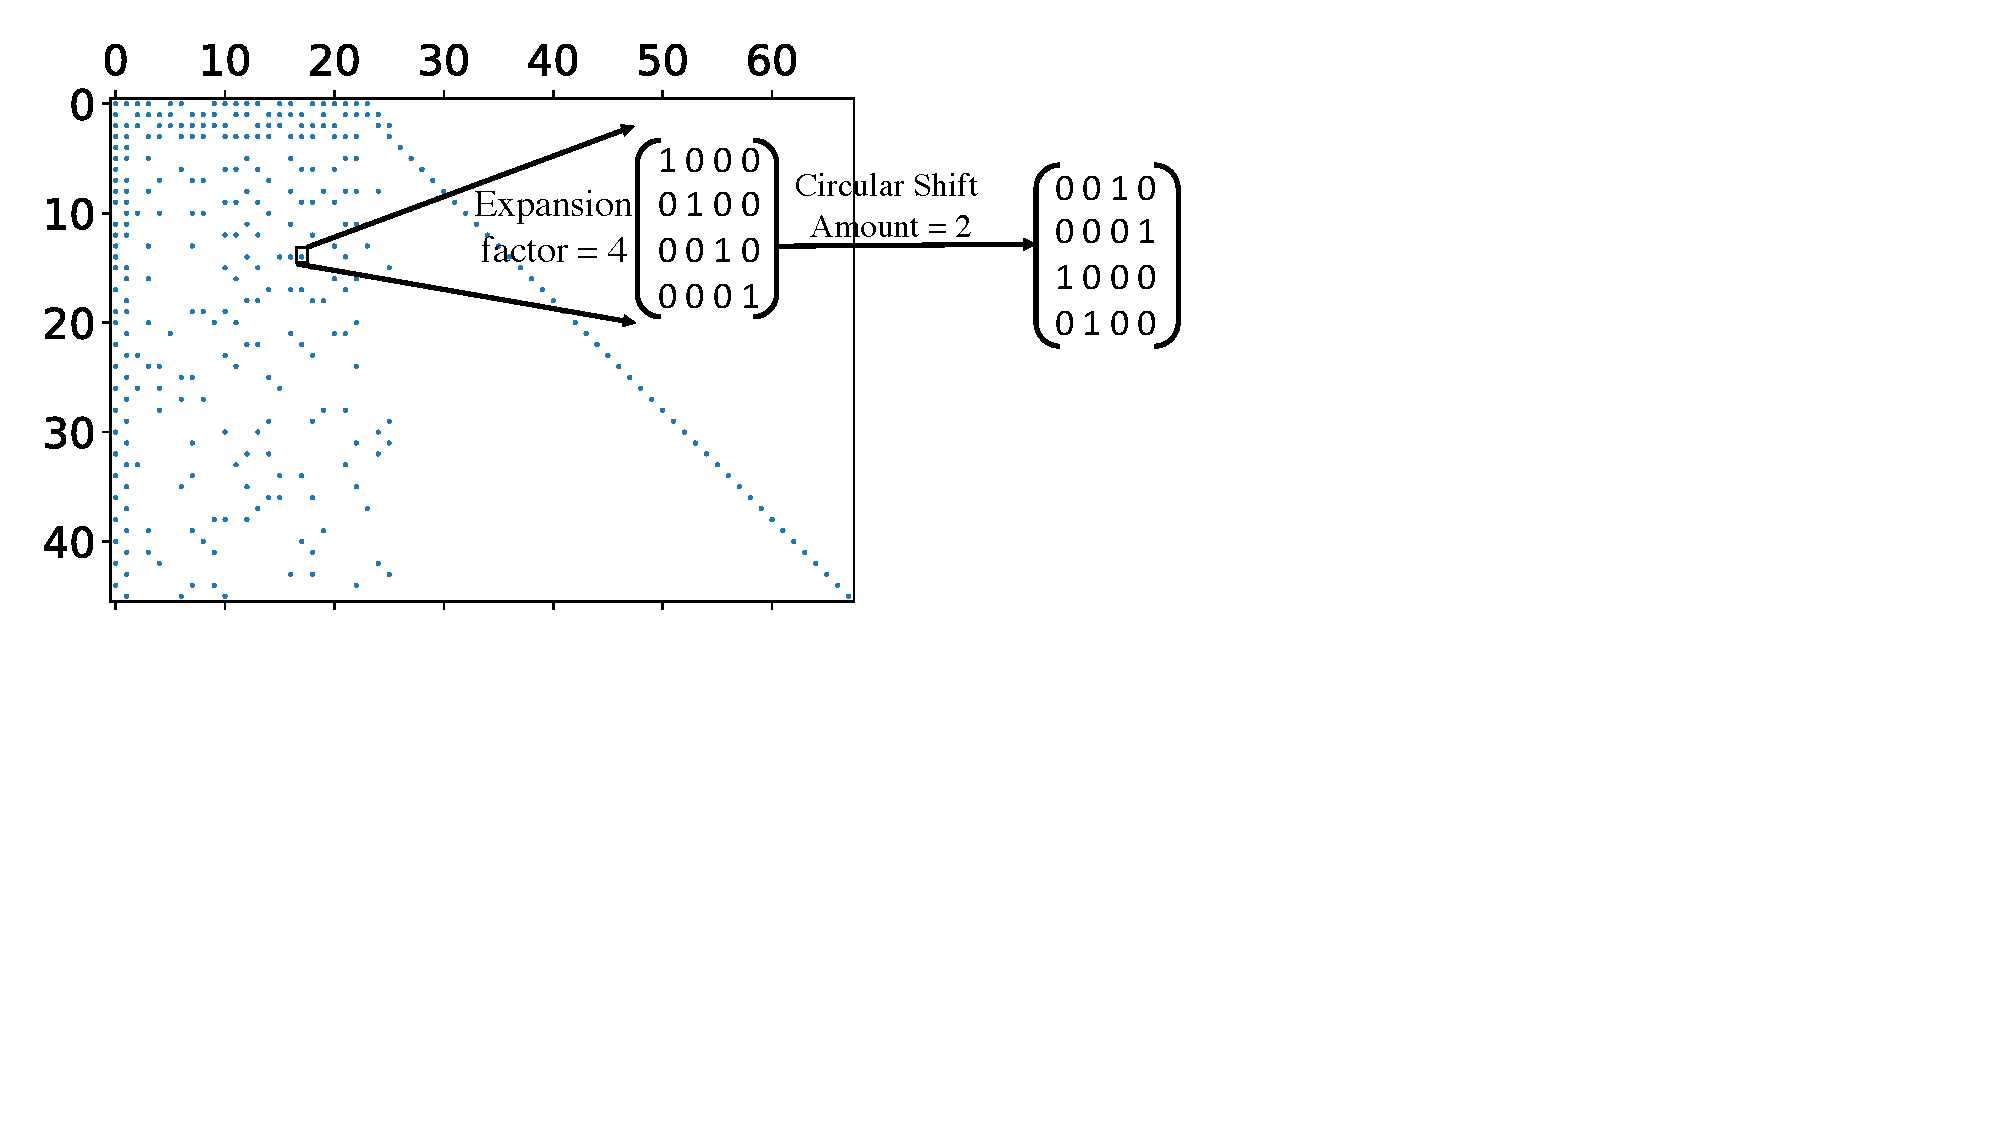
\includegraphics[width=1.9in]{FIGS/circular_shift.pdf}}
    \caption{Structure of 5G-NR standard base graph 1. Each blue dot represents a nonzero element which will be replaced by a circular identity matrix based on the expansion factor as shown.}
    \label{fig:5g-nr}
\end{wrapfigure}

Once the base graph is chosen, each zero entry is replaced with a $Z \times Z$ all-zero matrix. Each nonzero entry is replaced with a $Z \times Z $ circularly shifted identity matrix. $Z$ is called an expansion factor. The amount of circular shift depends on the value of the nonzero element. The values of the nonzero elements range from 0 to $Z-1$. If the value is 0, replace the element with the $Z \times Z$ identity matrix; otherwise, circularly shift the identity matrix based on the value. Fig.~\ref{fig:5g-nr} shows an example with an expansion factor of 4 and a circular shift amount of 2. The 5G-NR standard allows different discrete expansion factors ranging from 2 to 384. For further details, please refer to \cite{bae2019overview}.
\end{boxedminipage}
\end{figure}

\begin{figure}[htp]
    \centerline{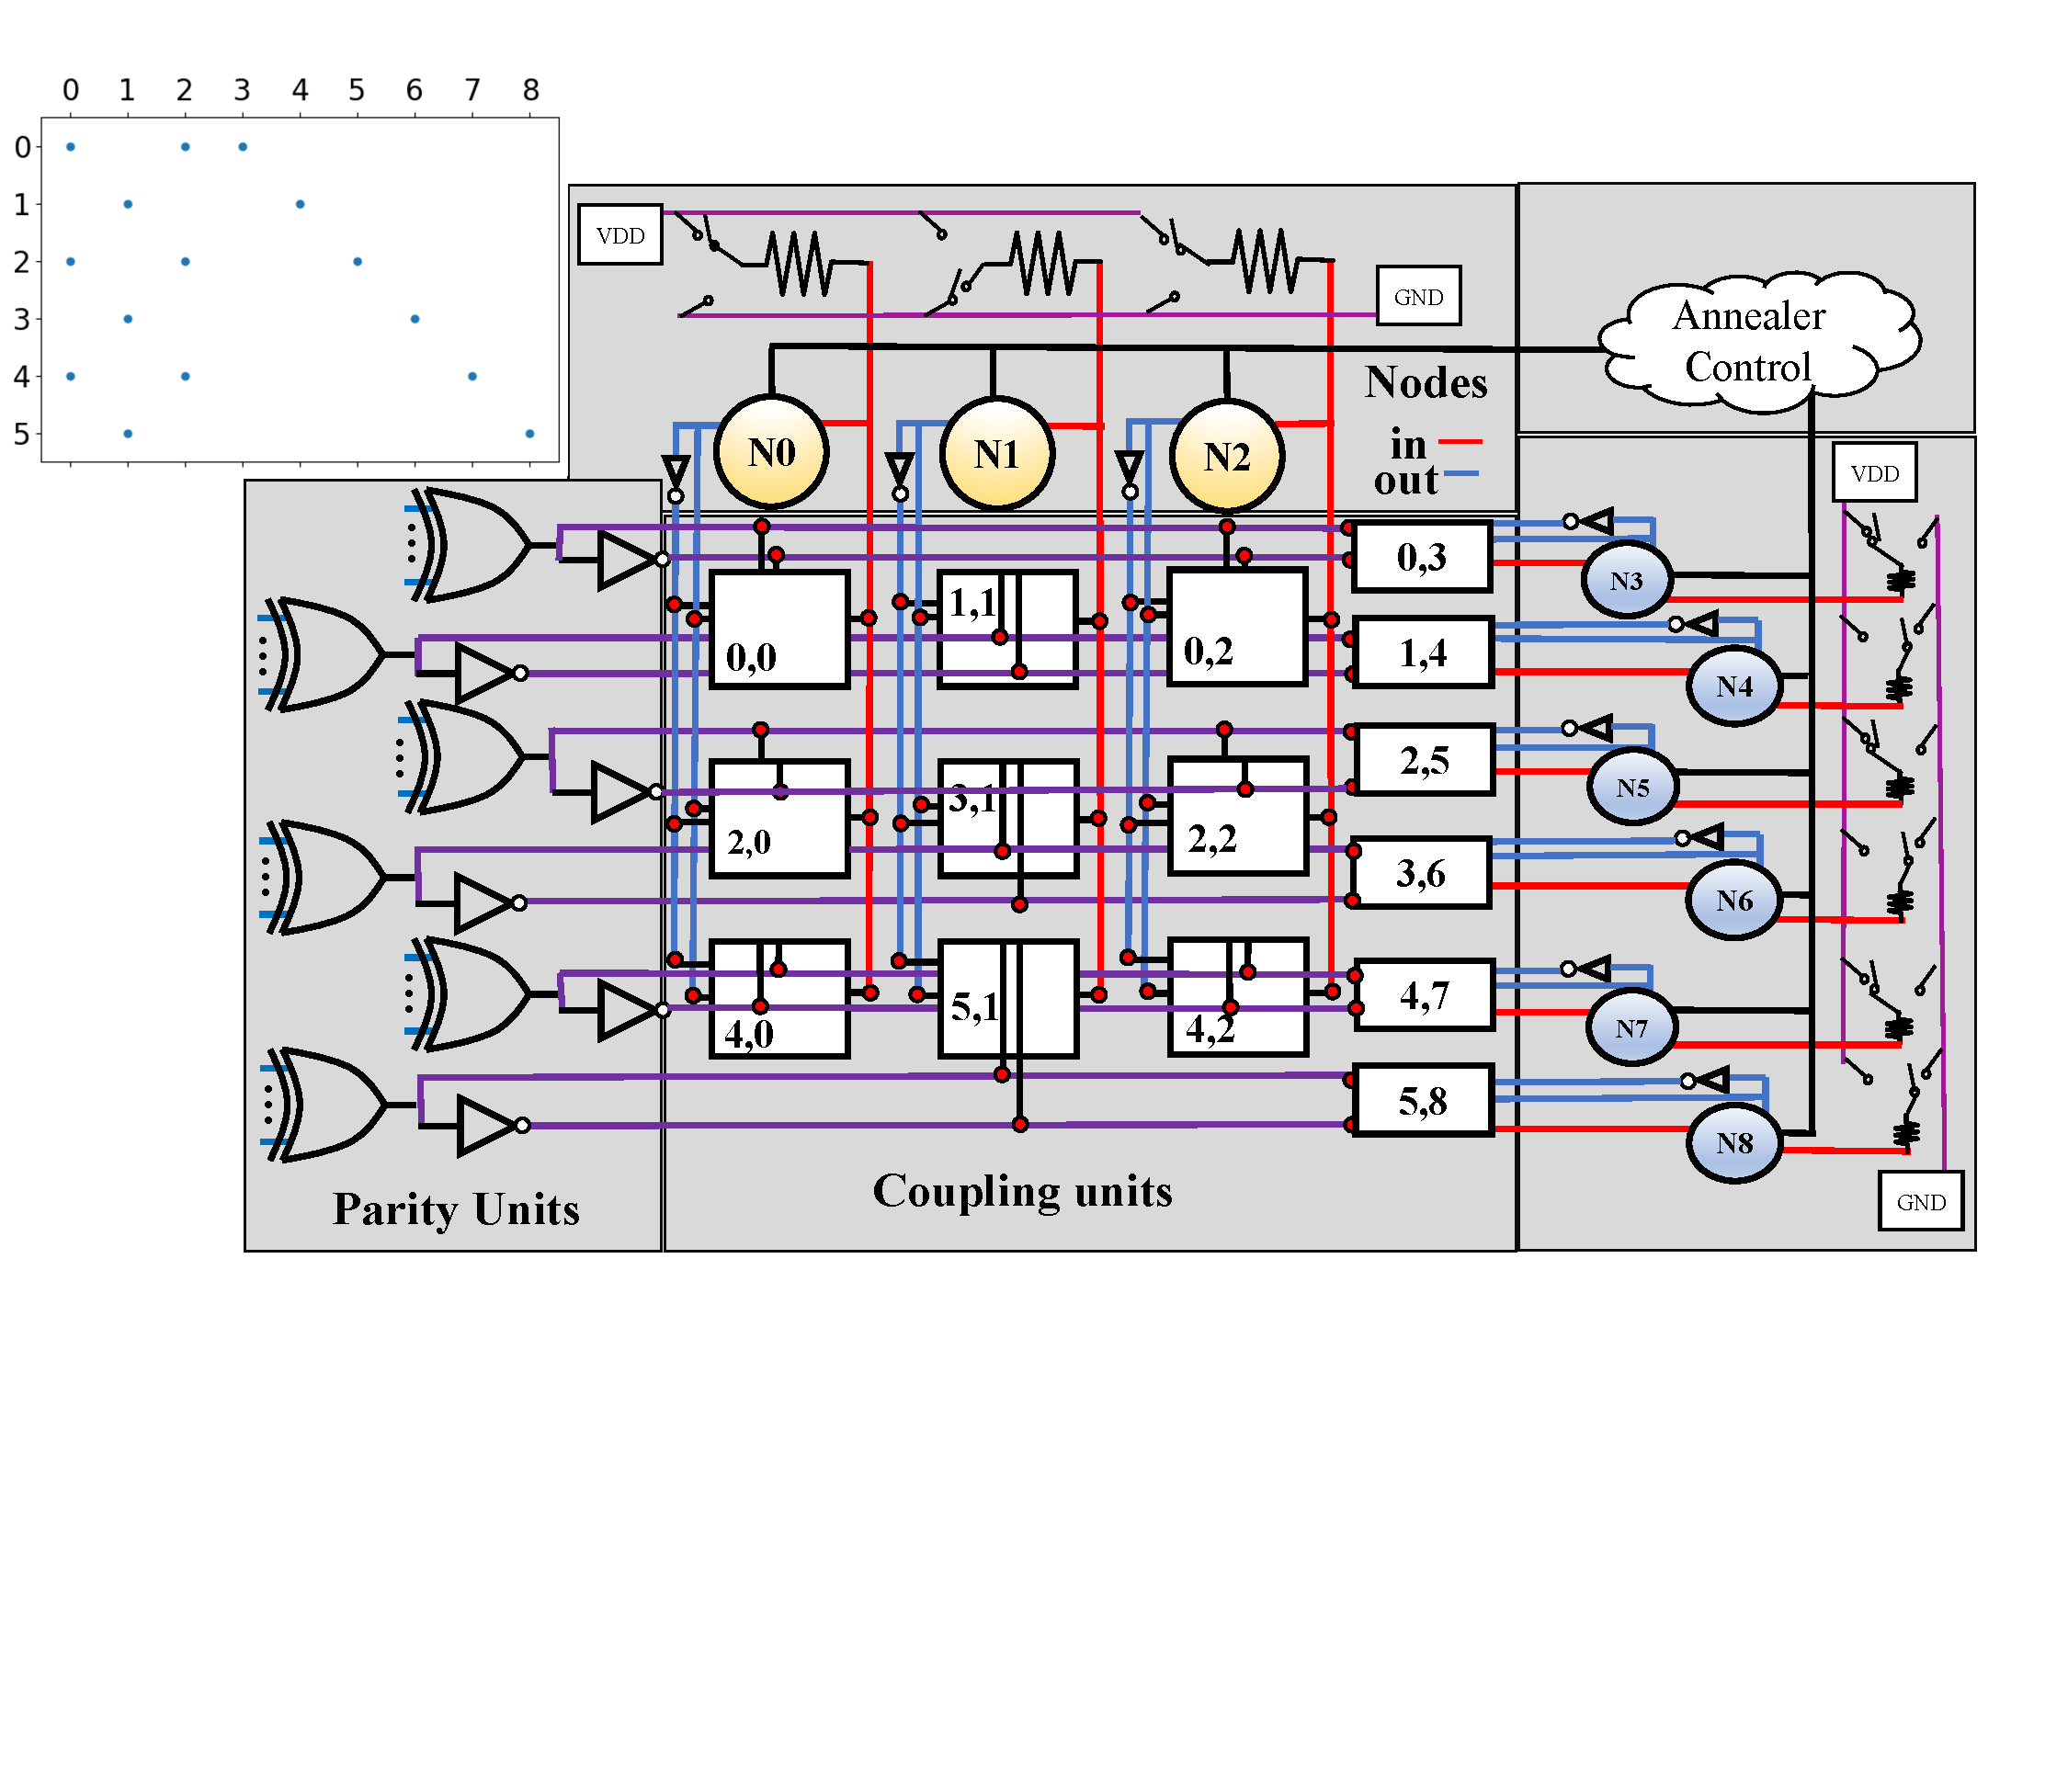
\includegraphics[width=0.50\textwidth]{FIGS/ldpc_arch_new_new1.pdf}}
    \caption{Illustration of our Ising machine-based LDPC decoder using a specific portion 
    (shown in top left) of the parity check matrix.} \label{fig:arch}
    %\todo{need to add pseudo matrix }
\end{figure}

\subsubsection{\bf Structure of the matrix}
As the name low-density suggests, the matrix is rather sparse, reducing the number of couplers
needed. A particular property of the 5G base matrix is that a large portion of the code bits
are only involved in a single parity check (so-called extension checks). In other words, many
columns (representing bits) have only one non-zero element. This portion is organized as a
diagonal submatrix and can be seen in Fig.~\ref{fig:5g-nr}. Because these spins have only one
coupler, their couplers can be easily incorporated into their node design. Overall, the coupling
array can be organized as a 2-d grid with auxiliary spins (parity checks) as one dimension
regular spins as another, with the checksum bit having single parities forming a special column.
The structure is shown in Fig.~\ref{fig:arch}.

To recap, with this architecture, the number of couplers equals the number of 1s in the
parity check matrix and is thus a constant (given a matrix), not affected by the number of
auxiliary spins we added. The auxiliary spins are generated from the XOR of all bits involved
in a parity check and thus have no degrees of freedom on their own. The state space of the
dynamical system is only a function of the number of regular spins.



\subsection{Circuit design}
\label{ssec:circuit}

\subsubsection{\bf Nodes}

In our baseline Ising machine~\cite{afoakwa.hpca21}, the spins are represented 
by voltage polarities on capacitors. %which are terminated to a \emph{virtual} ground (at half $V_{dd}$).
When representing $\sigma_i=+1$, corresponding to bit $\tilde{C_i}=0$,
the capacitor has a positive voltage.
Conversely, for $\sigma_i=-1$, its voltage is negative.

In the circuit implementation of the proposed Ising machine,
a spin is stored on a capacitor, and a node maintains the spin 
and interfaces with other circuits with its input/output circuit.
Fig.~\ref{fig:QuBRIM_node} shows an initial circuit design of a node. 
Besides the spin capacitor, it consists of three core functional blocks: 
a current conveyor, a one-bit quantizer, and a pair of spin-fix (SF) switches.
This node circuit takes an input current at $IN$, and generates an output voltage at $OUT$. 
The $OUT$ port of a node carries quantized voltage signals to both parity units and coupling units. 
The $IN$ port receives currents from coupling units. 
The node output can also be stored synchronously as a bit by an additional D flip-flop (DFF) when necessary.

%\begin{figure}[htp]
%\centering
%\includegraphics[width=0.30\textwidth]{LDPC codes/FIGS/qubrim_node.pdf}
%\caption{Circuit implementation of Node of LDPC decoder.} \label{fig:QuBRIM_node}
%\end{figure}

The current conveyor is constructed as a class-AB current mirror~\cite{kawahito1996cmos} %\cite{see Team QuiCC referenc}, 
which is designed for high slew rate and large input dynamic range. 
$M_5$-$M_8$ convey the input current from port $IN$ to node $Z$, 
hence charging/discharging the capacitor. 
The two current sources $I_{bias}$ set the bias condition for $M_1$-$M_4$, 
and hence the operating-point voltage at $Y$ is equal to that at $X$. 
By biasing node $X$ to $V_X=1/2(V_{DD}-V_{SS})$, 
$V_Y$ is effectively biased to the same voltage. 
The input impedance (at port $IN$) of this circuit is low,
allowing port $IN$ to operate as a current input.

\begin{wrapfigure}{r}{1.7in}
     {\includegraphics[width=1.7in]{FIGS/qubrim_node.pdf}}
     \caption{Circuit implementation of Node of LDPC decoder.}
     \label{fig:QuBRIM_node}
\end{wrapfigure}

The capacitor's voltage at node $Z$ represents the spin state: 
$V_Z<V_X$ for $\sigma_i=-1$, and $V_Z>V_X$ for $\sigma_i=+1$.
Note that this voltage $V_Z$ is an \emph{analog} signal, and needs to be quantized 
before it is used as an input for the XNOR gates in the parity and coupling units. 
Since our system operates in continuous-time, 
this quantizer can be simply constructed with inverters in series. 
In Fig.~\ref{fig:QuBRIM_node}, $M_{9-12}$ function as both a quantizer and super-buffer.

In order to configure the system's initial spins, 
%before the machine's states are allowed to evolve in seeking an energy minimum
two switches ($S_{1,2}$) are connected to node $Z$ to set/reset it to $V_{DD}$ or $V_{SS}$. 
We can also use these two switches to perform spin-fix perturbations, 
which allow the machine to escape local minima in search of the optimal solution. 
$SF_i^+$ and $SF_i^-$ are two non-overlapping control signals generated by the \emph{Annealer Control} unit.

\subsubsection{\bf Auxiliary spins and couplings}



For the auxiliary spins represent parity checks, 
let us consider the concrete case of checksum $j=0$ in Eq.~\ref{eq:chksum_ex}
($\tilde{C_1} \xor \tilde{C_3}\xor \tilde{C_5}$)
(the spin-based representation is $(1-\sigma_1\sigma_3\sigma_5)/2$). 
The physical meaning of the coupling is quite straightforward: 
when $\tilde{C_1}\xor \tilde{C_3}\xor \tilde{C_5}=0$,
each node will receive one unit of current keeping the node in the same polarity.
Conversely, when $\tilde{C_1}\xor \tilde{C_3}\xor \tilde{C_5}=1$, each node will
receive one unit of current trying to change the polarity of the node. 
We achieve this by generating the checksum ($\tilde{C_1}\xor\tilde{C_3}\xor \tilde{C_5}$)
to select for each spin whether to couple to its positive or negative edge of its own
node. An alternative view is that the selector acts as an additional XOR gate to
``back out" its own node. Thus, for node 1, the coupling comes from 
$\tilde{C_1} \xor \tilde{C_3}\xor \tilde{C_5}\xor\tilde{C_1}=\tilde{C_3}\xor \tilde{C_5}$.
%\begin{wrapfigure}{r}{3in}
%    {
\includegraphics[width=3in]{LDPC codes/FIGS/circuit_diagram_ldpc_pass.pdf}}
%    \caption{Logical implementation of proposed LDPC decoder.}
%    \todo{show the new pass gate based coupling controlled by a single auxiliary spin. Also use the
%    same orientation as the matrix}
%    \label{fig:circuit_digaram}
%\end{warpfigure}

\begin{figure}[htp]
\centerline{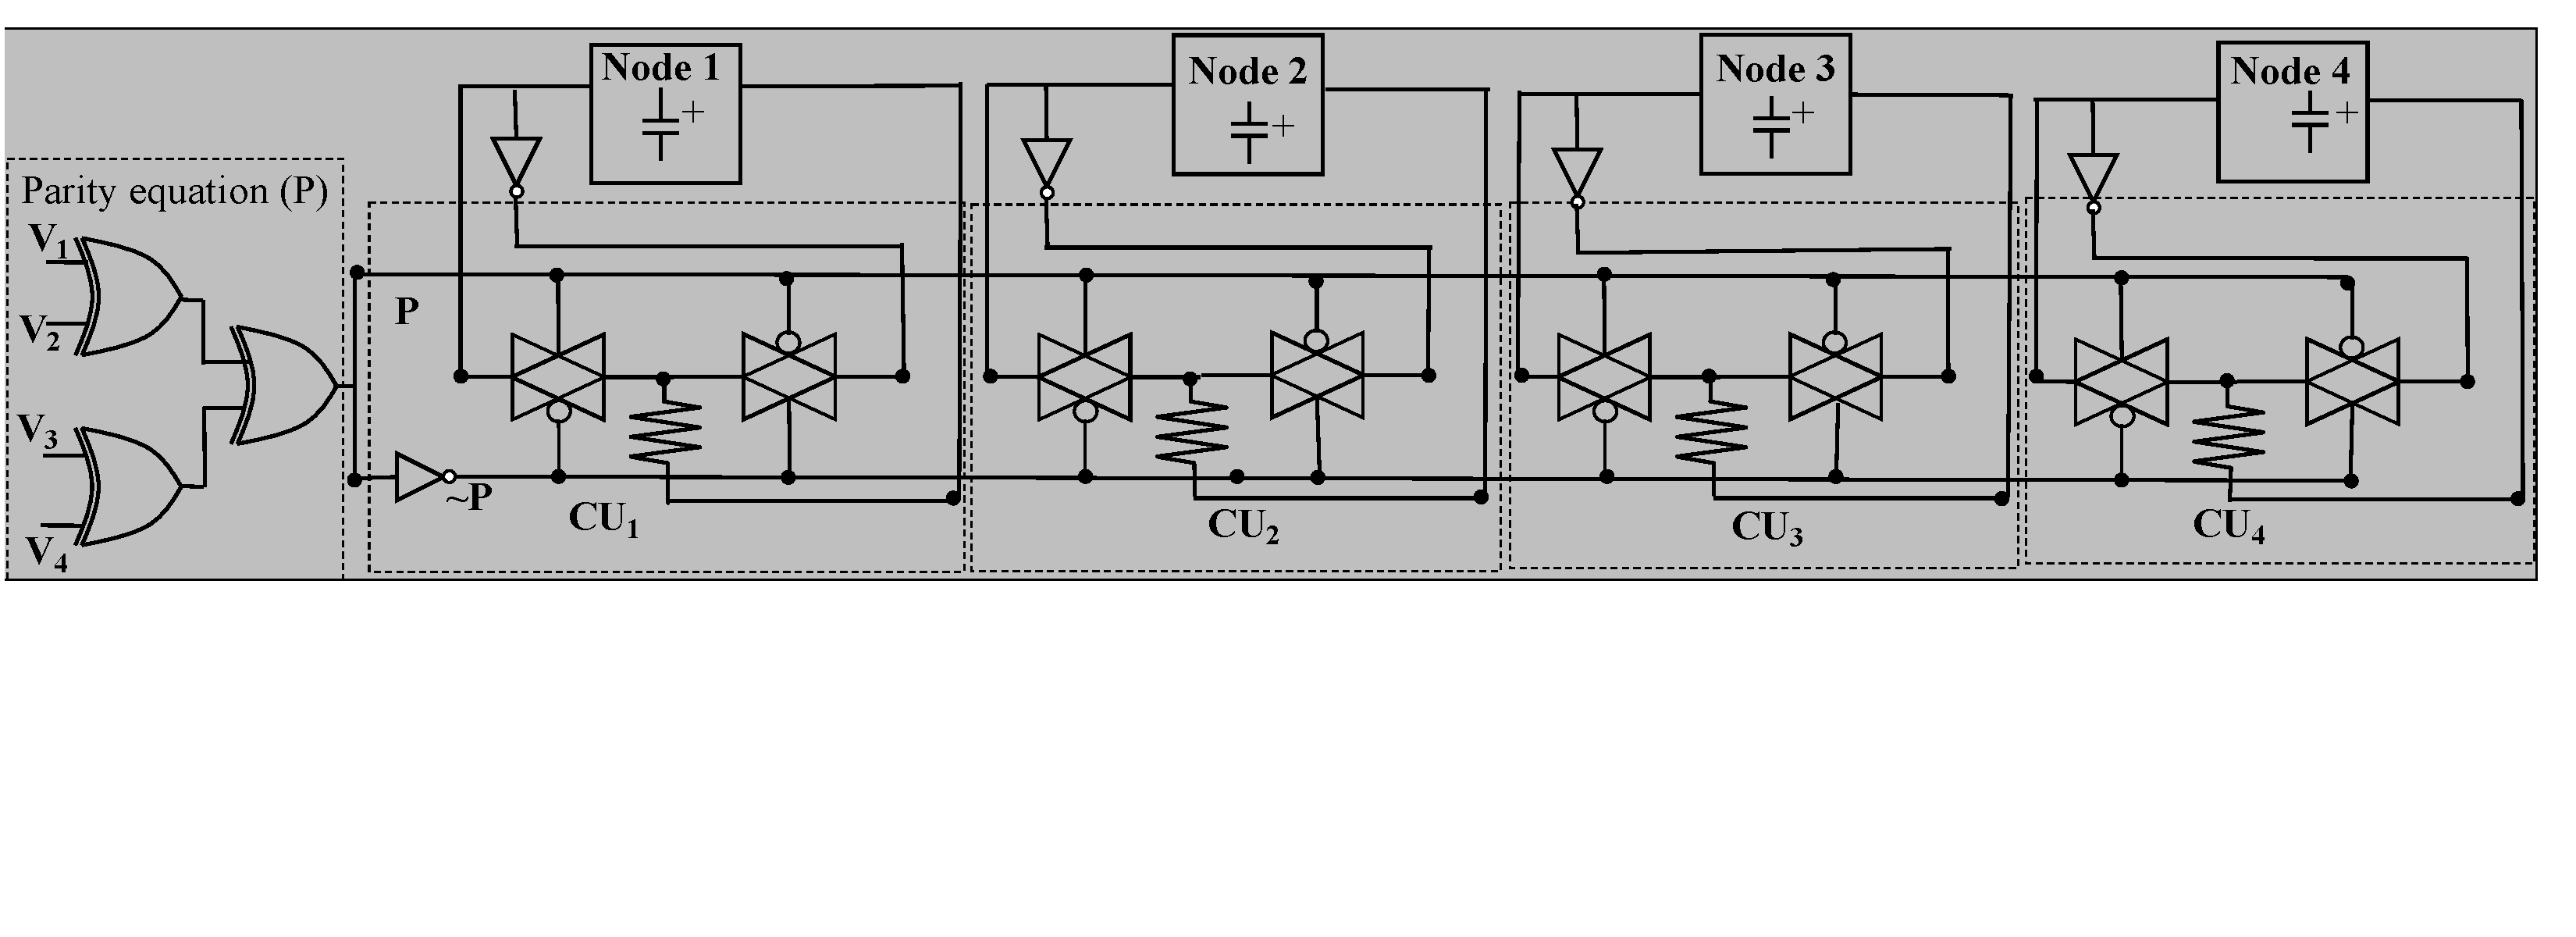
\includegraphics[width=0.5\textwidth]{FIGS/circuit_diagram_ldpc_pass.pdf}}
    \caption{Circuit implementation of parity check and its coupling to spins.} \label{fig:circuit_digaram}
\end{figure}

    %\todo{show the new pass gate based coupling controlled by a single auxiliary spin. Also use the same orientation as the matrix}
%We apply an additional optimization to reduce circuitry. This is best explained through an example. Let us assume row $j$ of $H$ has 4 non-zero elements, which we will simply refer to as Nodes 1 to 4. As the discussion above shows, each node will need an auxiliary spin that is the result of XOR of the other three nodes, \eg Node 2 will couple with the XOR of Nodes 1, 3, 4. This can be easily done by generating the XOR of all four nodes and then ``back out", say, Node 1 (by XOR'ing with it again) just before coupling with Node 1's capacitor.  Fig.~\ref{fig:circuit_digaram} shows the circuit.


%\subsubsection{\bf Parity, Coupling, and Bias Units}   Parity units represent the parity check equations or rows of a parity check matrix. As our design hardwires a particular parity check matrix, parity units are a binary tree of XNOR gates. These units are used to evaluate $P_j$ in the Equation~\ref{eq::LDPC_ising}. For the base graph 1 of the 5G standard, the maximum number of nodes involved in a parity check equation is 19; hence the maximum height of the binary tree will be five stages. As shown in the Figure~\ref{fig:arch} the output of each parity unit is fed into the columns of coupling units if a node ($N_i$) is involved in a parity check equation ($P_j$), the coupling unit ($CU_{i,j}$) is used for coupling the parity equation with the node. The coupling unit consists of an XNOR gate and a resistor. The output of the XNOR gate is connected to the $IN$ terminal of the node through a resistor. It determines the value of $P_{j \backslash i}$ and passes it to node $N_i$. The value of the resistor varies according to the $\alpha$ value. The bias represents the linear term in the Equation~\ref{eq::LDPC_ising}. It is implemented as a resistor connected to either VDD or GND, depending upon the sign of $R$. The absolute value of $R$ determines the value of the resistor.

\subsubsection{\bf Bias}
The linear terms ($-2R_i\sigma_i$ in Eq.~\ref{eq::LDPC_ising}) helps to 
constrain the decoded output closer to the received message, and is implemented by a 
bias current at each node proportional to the received value $R_i$. 
More specifically, according to Eq.~\ref{eq::LDPC_ising}, the bias current for
node $i$ needs to be $\frac{4R_i}{\alpha}$ time that of the coupling current from
the parity check. The sign of $R_i$ determines the polarity of the bias current. 

Putting everything together, 
Eq.~\ref{eqn:rim_node_simplifed} describes the circuit behavior.
We can see that if we use voltage $v_i$ (relative to virtual ground) 
as an approximation for spin $\sigma_i$ in Eq.~\ref{eq::LDPC_ising}, 
Eq.~\ref{eqn:rim_node_simplifed} is proportional to the gradient.
\begin{equation}\label{eqn:rim_node_simplifed}
\begin{split}
%    \dv{v_i}{t} = \frac{1}{C}(I_{in}) =  \frac{1}{C} \left[ \sum_{\mathclap{j}} J_{ij}*(P_{j\backslash i}) + {J_b}_i*({v_b}_i) \right]
    \dv{v_i}{t} = \frac{1}{C}(I_{in}) =  \frac{1}{C} \left[ \sum_{\mathclap{j}} J_{ij}*(P_{j\backslash i}) + {J_b}_i*({v_b}_i) \right] \\
    \dv{v_i}{t} = \frac{J}{C}(I_{in}) =  \frac{J}{C} \left[ \frac{4R_i}{\alpha}*{v_b}_i  + 
    \sum_{\mathclap{H_{j,i}=1}} \sigma_{j\backslash i} \right]
\end{split}
\end{equation}

 %As shown in Fig ~\ref{fig:PU} an XNOR gate (X1) with inputs $V_i+$ and $P_j^{in}$ are used to determine function \ding{172}. The output of the gate X1 is connected to $V_i-$ via a programmable coupling resistor ($T_1$) which acts as a switch. The programmable coupling resistor is implemented using a transistor whose charge on gate capacitance determines if the switch is on or off. According to parity equation $P_j$, if node $V_i$ is involved, then the switch $T_1$ would be turned on; otherwise, off. \ding{173} function is implemented using another XNOR gate (X2). As shown in Fig ~\ref{fig:PU} the inputs of XNOR (X2) gate are $P_j^{out}$ and $V_i+$.  $P_j^{out}$ represents the value of the parity equation ($P_j$) determined by the previous nodes in the column. If node $V_i$ is involved in the equation, then the node's current state should be XNORed with $P_j^{out}$ to determine the final value. If it is not involved in the equation, we should pass the value on to other nodes. To implement this, we used two switches $T_2$ and $T_3$ operating conversely. If node $V_i$ is involved then $T_2$ is turned on and $T_3$ is off; otherwise $T_3$ is turned on and $T_2$ is left off. These coupling resistors are programmed using a row selector and a column selector, which will be discussed in the next section. After determining the final value of $P_j$, it is passed as input to the parity units to calculate $P_j\backslash i$. The nodes c1, c2, and c3 in Figure~\ref{fig:BRIM_arch} represent the connection of wires between the $P_j^{out}$ and $P_j^{in}$. In this way, we have changed the architecture, nodes, and coupling unit structure of BRIM to directly map the LDPC decoding problem to the system. The rest of the unit's functionality is the same as BRIM, but we discuss it here also.
%Figure~\ref{fig:arch} shows architecture design of our LDPC decoder for a  base graph with 3 rows and 4 columns and for an expansion factor of 4. It has three main architectural components, \ding{172}  Node units blocks (N1 to Nn), \ding{173} parity units Block, \ding{174} check nodes units block (CNB1 to CNB3). The shaded regions represent zero elements in the base graph. Each block is replaced with an array of units based on the expansion factor as shown in figure. These units are hardwired based on the parity check matrix. The rows in~\ref{fig:arch} represent columns of the base graph and vice versa.
%Row $i$ are used for calculating $\sum_j P_{j\backslash i}$ of a node $i$ by summing the output currents from parity units of that row. Column $j$ is used to evaluate the parity equation "$P_j$." 

\begin{comment}    

\subsubsection{\bf Nodes}

We slightly modified bistable nodes $v_i$ of BRIM to implement biasing. In Fig.~\ref{fig:node_and_iv} we show a more detailed illustration of one node. A ZIV diode is used as the feedback circuit to stabilize the voltages at the desired levels (\eg $\pm V_{dd}$). The figure shows the IV curve of the ZIV diode. When capacitor voltages are in between $-V_{dd}$ and $V_{dd}$, the diode acts as an active element charging its voltage closer to $\pm V_{dd}$. Conversely, for voltages outside the range, the ZIV diode acts essentially as a linear resistor to discharge the capacitor. 

Each node is supplied with two pairs of switches to set the capacitor voltage to a known spin state. It is helpful for specific initialization or to change the system state as described in the  "Annealing Control "(Sec.~\ref{ssec:anneal_control}). Finally, the spin of the node can be read 
out by a digital latch (\eg a D flip-flop) connected to the ZIV diode's 
$V+$ terminal. It converts the spin to a bit (1 or 0). The pins labeled $V+$, and $V-$ are used to connect to the parity units' inputs and outputs. The bias determined by the received message is applied as a voltage through resistors (B+, B-) as shown in figure~\ref{fig:node_and_iv}. The value of resistance depends upon the value and sign of the received message.

\begin{figure}[htp]\centering
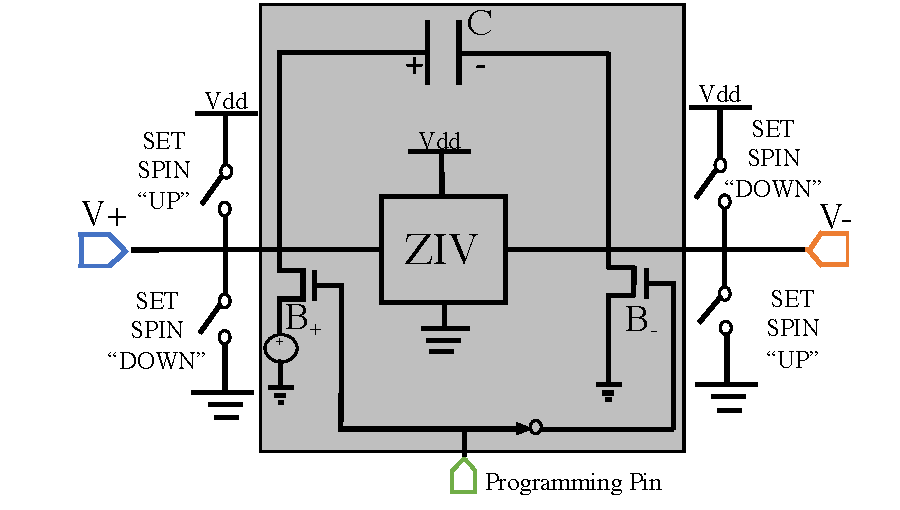
\includegraphics[width=0.28\textwidth]{FIGS/variable_node.pdf}

\includegraphics[width=0.20\textwidth]{ziv_curve.pdf}
\caption{Simplified schematic of one BRIM node (left) and ZIV diode's IV 
characteristic (right). \label{fig:node_and_iv}}
\end{figure}

\subsubsection{\bf Parity Unit}

The parity unit ($PU_{ij}$) represents the coupling unit in BRIM. Here, it is used for coupling node $V_i$ to parity equation $P_j$ and vice versa. It has the following functionalities \ding{172} to determine value $P_{j \backslash i}$ and pass it to node $V_i$ ,\ding{173} to evaluate the parity equation $p_j$ if node $V_i$ is connected to parity equation $P_j$, otherwise just pass the previous value of $P_j$ value to other nodes in same column.

 As shown in Fig ~\ref{fig:PU} an XNOR gate (X1) with inputs $V_i+$ and $P_j^{in}$ are used to determine function \ding{172}. The output of the gate X1 is connected to $V_i-$ via a programmable coupling resistor ($T_1$) which acts as a switch. The programmable coupling resistor is implemented using a transistor whose charge on gate capacitance determines if the switch is on or off. According to parity equation $P_j$, if node $V_i$ is involved, then the switch $T_1$ would be turned on; otherwise, off. \ding{173} function is implemented using another XNOR gate (X2). As shown in Fig ~\ref{fig:PU} the inputs of XNOR (X2) gate are $P_j^{out}$ and $V_i+$.  $P_j^{out}$ represents the value of the parity equation ($P_j$) determined by the previous nodes in the column. If node $V_i$ is involved in the equation, then the node's current state should be XNORed with $P_j^{out}$ to determine the final value. If it is not involved in the equation, we should pass the value on to other nodes. To implement this, we used two switches $T_2$ and $T_3$ operating conversely. If node $V_i$ is involved then $T_2$ is turned on and $T_3$ is off; otherwise $T_3$ is turned on and $T_2$ is left off. These coupling resistors are programmed using a row selector and a column selector, which will be discussed in the next section. After determining the final value of $P_j$, it is passed as input to the parity units to calculate $P_j\backslash i$. The nodes c1, c2, and c3 in Figure~\ref{fig:BRIM_arch} represent the connection of wires between the $P_j^{out}$ and $P_j^{in}$. In this way, we have changed the architecture, nodes, and coupling unit structure of BRIM to directly map the LDPC decoding problem to the system. The rest of the unit's functionality is the same as BRIM, but we discuss it here also.
 
\begin{figure}[htp]
    \centerline{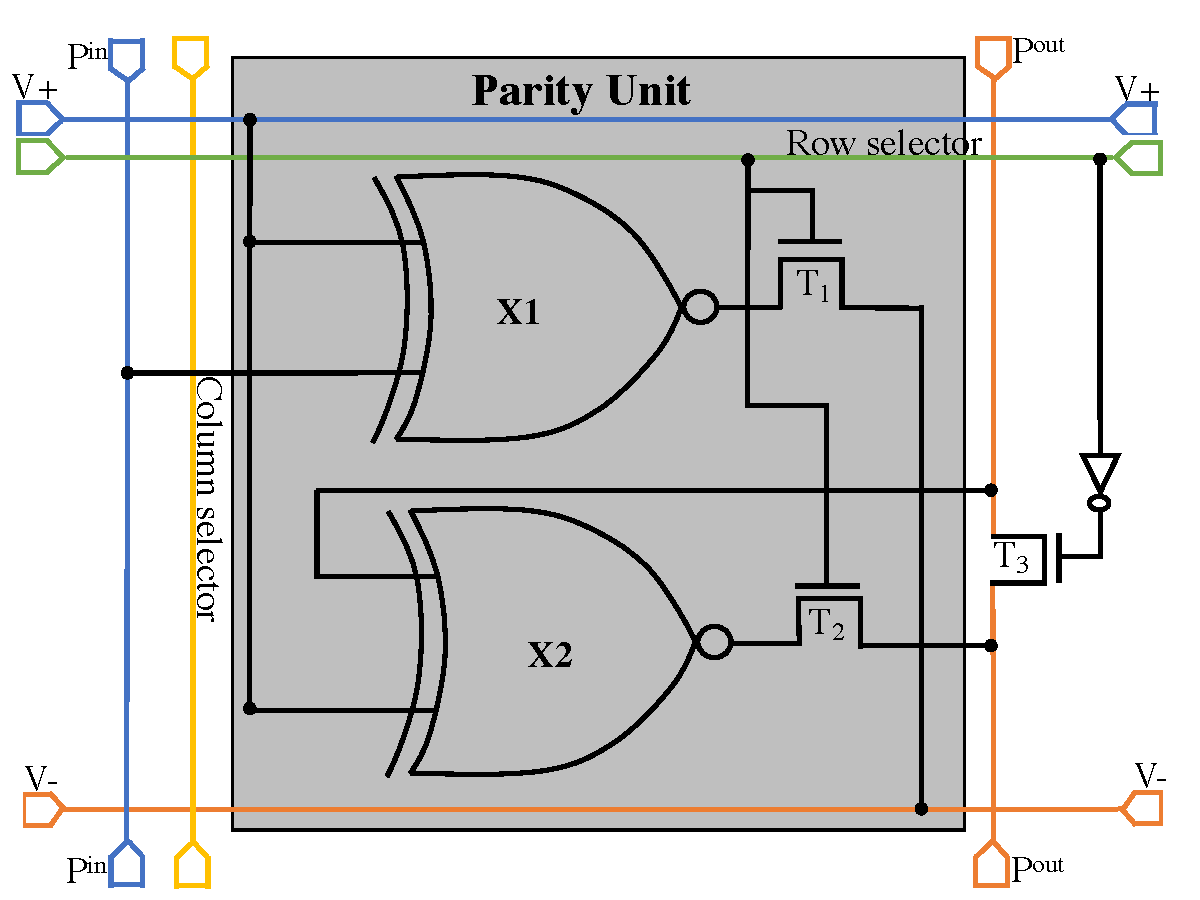
\includegraphics[width=0.5\textwidth]{FIGS/parity_unit_ldpc.pdf}}
    \caption{Schematic of parity unit. Color schemes are matched to system-level block diagram in Fig ~\ref{fig:arch} }
    \label{fig:PU}
\end{figure}

\end{comment}
%If the sign of the message is positive, switch B+ is turned on, and B- is turned off, and vice versa. These switches are programmed using the programming pin.
%\end{comment}

\begin{comment}
    

\subsubsection{\bf Programming units}
Both the initial nodal values and the coupling resistances in parity units are programmable.
Programming of a resistor is achieved through a transistor with adjustable 
gate voltage.
% The details of the circuit design are discussed in Appendix~\ref{ ssec:circuit}. 
To the right of the parity unit array in 
Fig.~\ref{fig:arch} is the programming array. This array consists of 
digital memory for storing the weights which drive an array of digital-to-analog 
converters (DACs).

A small amount of such DACs are sufficient to program all the parity units in a time-interleaved fashion per column. In such configuration, 
we need corresponding column selectors and pull-down logic as shown below 
the coupling units in Fig.~\ref{fig:arch}.

\subsubsection{\bf Annealing control}\label{ssec:anneal_control}

As our system is primarily an optimizer, it can get stuck in local minima. To avoid this, two commonly used mechanisms for annealers were adopted and incorporated to allow the system to escape local optima. First, the coupling strength is globally increased over time. In this way, at the very beginning, the machine is only weakly coupled, rendering the energy landscape relatively flat. It helps the system explore the landscape in a coarse granularity. We choose an exponential annealing schedule because (a) it is a common practice, and (b) it can be conveniently achieved by discharging an appropriately-sized capacitor as the global annealing scheduler. The voltage from this capacitor is then used to control the variable gain buffer in each node to achieve the change in coupling strength.

Second, we adopt a similar strategy as that used in simulated annealing. In Simulated annealing, the spins are flipped based on a probability decided by the differences in the energy. Doing the same thing in hardware is a complex process. To simplify the process, we use a "spin fix"; we randomly choose a node and briefly clip it to one of the supply rails. The nodal spin either maintains its current state or swaps to the opposite state. The probability/frequency of spin fixes is determined based on temperature. The temperature follows the same exponential annealing schedule discussed above. In other words, the frequency of spin fixes decays exponentially over time.
\end{comment}

%\subsection{Theoretical analysis}
%\todo{needs to be changed}
%We can theoretically define the evolution of above described LDPC decoder using equation~\ref{eqn:rim_node_simplifed}. It shows how the voltage of a capacitor representing each node change over time. $J_{ij}$ represents the effective conductance of the coupling with the parity equations. $B_i$ represents the bias current representing the bias term in the equation~\ref{eq::LDPC_ising}. %and  $g_{\!_{ZIV}}(v_{i})$ represents the current due to $ZIV$ diode.
%\begin{equation}\label{eqn:rim_node_simplifed}
%\begin{split}
%    \dv{v_i}{t} = \frac{1}{C}(I_{in} - I_{ZIV}) =  \frac{1}{C} \left[ \sum_{\mathclap{j}} J_{ij} P_{j\backslash i} + B_i  \right]
%\end{split}
%\end{equation}
%With this equation, we can provide the same Lyapunov stability analysis as shown in the following paper~\cite{afoakwa.hpca21} to prove our ability for optimum-seeking

\begin{comment}

\subsection{Architecture of hybrid LDPC decoder}
\label{ssec:arch}

We now discuss the architectural changes made to BRIM to implement an LDPC decoder. The system is illustrated in Fig.~\ref{fig:BRIM_arch} and consists of: 
\ding{172} bistable nodes (V1 to V4) and their digital interface (DFF 1-4); 
\ding{173} parity units connecting the nodes ($PU_{ij}$); \ding{174} 
programming units to configure parity units (including: memory, multiplexers,
digital-to-analog converters, and the column control systems); and \ding{175} annealing control. The rows (i) represent the variable nodes, and the columns (j) represent check nodes in a Tanner graph. Row $i$ is used for calculating $\sum_j P_{j\backslash i}$ of a node $i$ by summing the output currents from parity units of that row. Column $j$  is used to evaluate the parity equation "$P_j$." We discuss each unit in turn as follows:

\begin{figure}[htp]
    \centerline{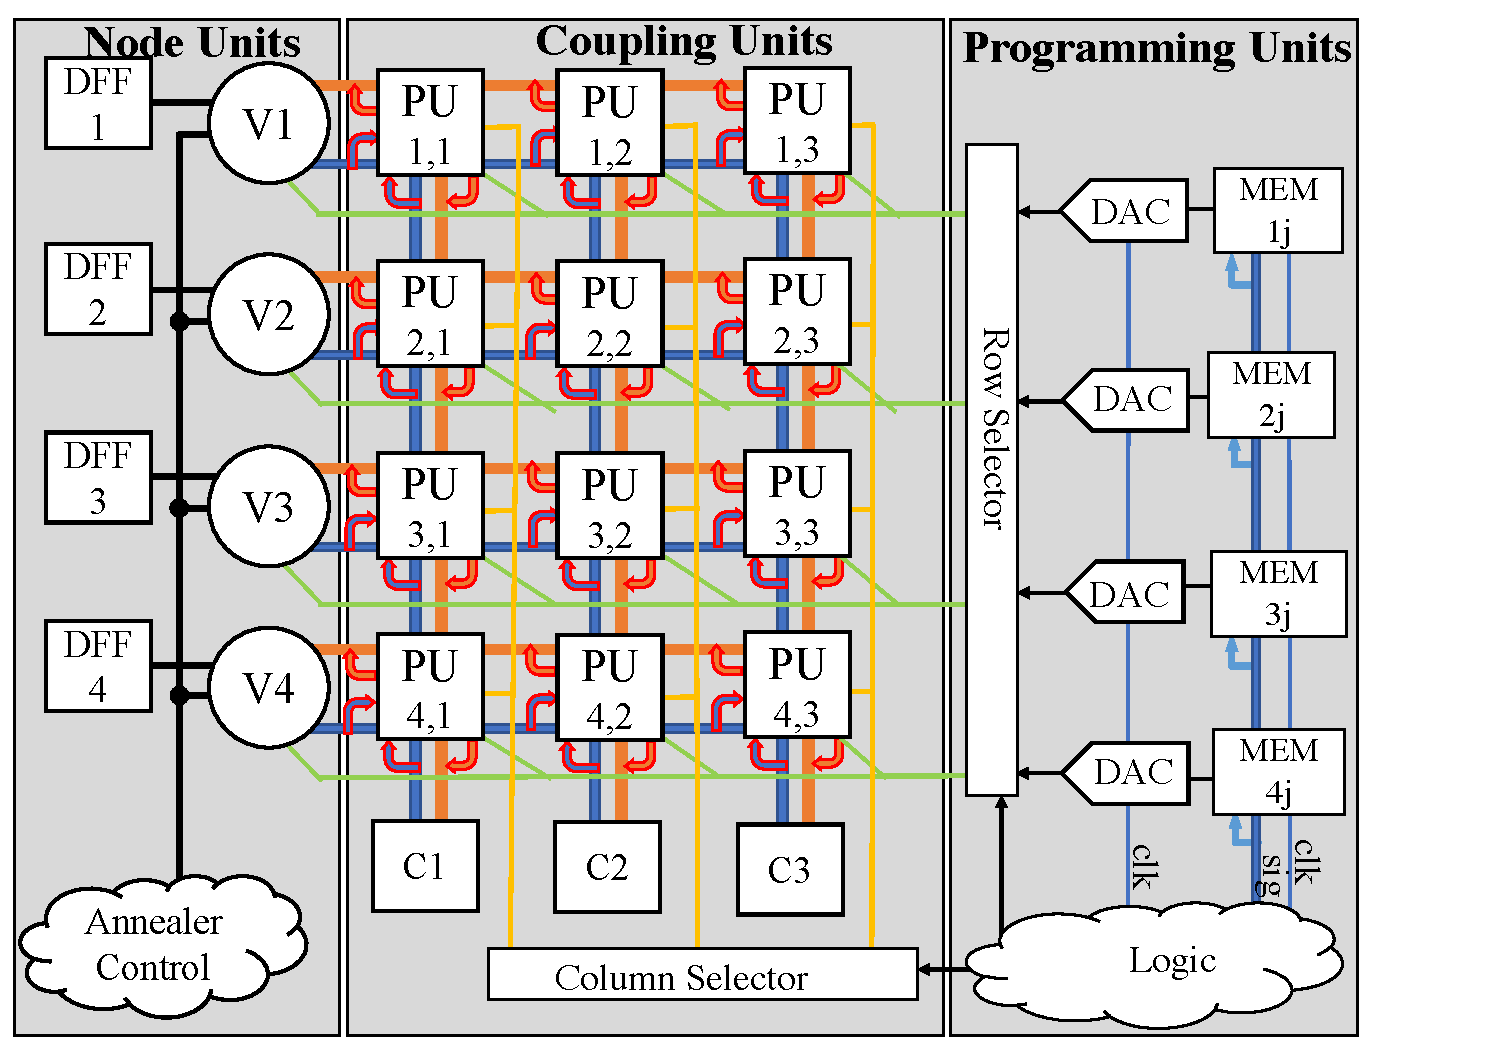
\includegraphics[width=0.45\textwidth]{FIGS/ldpc_new_arch.pdf}}
    \caption{Block diagram of BRIM based LDPC decoder's system components. Nodes are $N_i$ and parity units $PU_{i,j}$. The multi-colored interconnecting links are wires}
    \label{fig:BRIM_arch}
\end{figure}

\subsubsection{\bf Nodes}

We slightly modified bistable nodes $v_i$ of BRIM to implement biasing. In Fig.~\ref{fig:node_and_iv} we show a more detailed illustration of one node. A ZIV diode is used as the feedback circuit to stabilize the voltages at the desired levels (\eg $\pm V_{dd}$). The figure shows the IV curve of the ZIV diode. When capacitor voltages are in between $-V_{dd}$ and $V_{dd}$, the diode acts as an active element charging its voltage closer to $\pm V_{dd}$. Conversely, for voltages outside the range, the ZIV diode acts essentially as a linear resistor to discharge the capacitor. 

Each node is supplied with two pairs of switches to set the capacitor voltage to a known spin state. It is helpful for specific initialization or to change the system state as described in the  "Annealing Control "(Sec.~\ref{ssec:anneal_control}). Finally, the spin of the node can be read 
out by a digital latch (\eg a D flip-flop) connected to the ZIV diode's 
$V+$ terminal. It converts the spin to a bit (1 or 0). The pins labeled $V+$, and $V-$ are used to connect to the parity units' inputs and outputs. The bias determined by the received message is applied as a voltage through resistors (B+, B-) as shown in figure~\ref{fig:node_and_iv}. The value of resistance depends upon the value and sign of the received message.

%If the sign of the message is positive, switch B+ is turned on, and B- is turned off, and vice versa. These switches are programmed using the programming pin.

\begin{figure}[htp]\centering
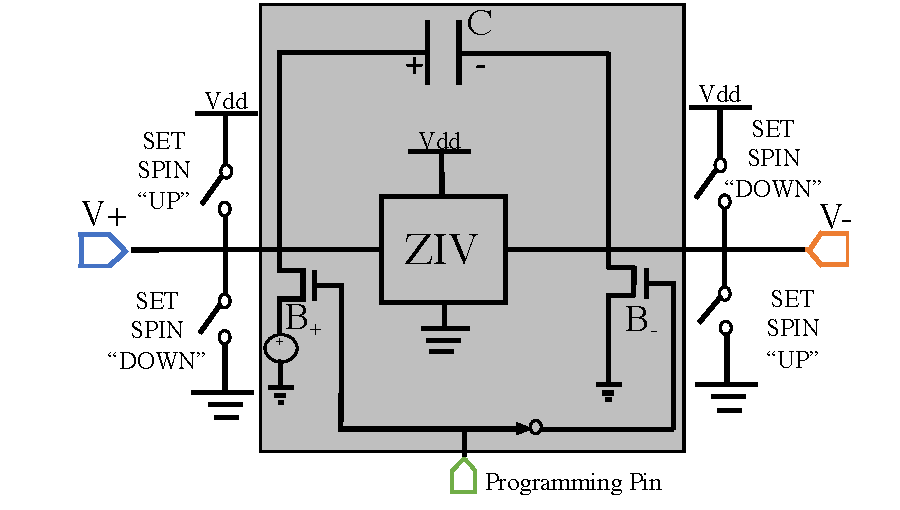
\includegraphics[width=0.28\textwidth]{FIGS/variable_node.pdf}

\includegraphics[width=0.20\textwidth]{ziv_curve.pdf}
\caption{Simplified schematic of one BRIM node (left) and ZIV diode's IV 
characteristic (right). \label{fig:node_and_iv}}
\end{figure}

\subsubsection{\bf Parity Unit}

The parity unit ($PU_{ij}$) represents the coupling unit in BRIM. Here, it is used for coupling node $V_i$ to parity equation $P_j$ and vice versa. It has the following functionalities \ding{172} to determine value $P_{j \backslash i}$ and pass it to node $V_i$ ,\ding{173} to evaluate the parity equation $p_j$ if node $V_i$ is connected to parity equation $P_j$, otherwise just pass the previous value of $P_j$ value to other nodes in same column.

 As shown in Fig ~\ref{fig:PU} an XNOR gate (X1) with inputs $V_i+$ and $P_j^{in}$ are used to determine function \ding{172}. The output of the gate X1 is connected to $V_i-$ via a programmable coupling resistor ($T_1$) which acts as a switch. The programmable coupling resistor is implemented using a transistor whose charge on gate capacitance determines if the switch is on or off. According to parity equation $P_j$, if node $V_i$ is involved, then the switch $T_1$ would be turned on; otherwise, off. \ding{173} function is implemented using another XNOR gate (X2). As shown in Fig ~\ref{fig:PU} the inputs of XNOR (X2) gate are $P_j^{out}$ and $V_i+$.  $P_j^{out}$ represents the value of the parity equation ($P_j$) determined by the previous nodes in the column. If node $V_i$ is involved in the equation, then the node's current state should be XNORed with $P_j^{out}$ to determine the final value. If it is not involved in the equation, we should pass the value on to other nodes. To implement this, we used two switches $T_2$ and $T_3$ operating conversely. If node $V_i$ is involved then $T_2$ is turned on and $T_3$ is off; otherwise $T_3$ is turned on and $T_2$ is left off. These coupling resistors are programmed using a row selector and a column selector, which will be discussed in the next section. After determining the final value of $P_j$, it is passed as input to the parity units to calculate $P_j\backslash i$. The nodes c1, c2, and c3 in Figure~\ref{fig:BRIM_arch} represent the connection of wires between the $P_j^{out}$ and $P_j^{in}$. In this way, we have changed the architecture, nodes, and coupling unit structure of BRIM to directly map the LDPC decoding problem to the system. The rest of the unit's functionality is the same as BRIM, but we discuss it here also.
 
\begin{figure}[htp]
    \centerline{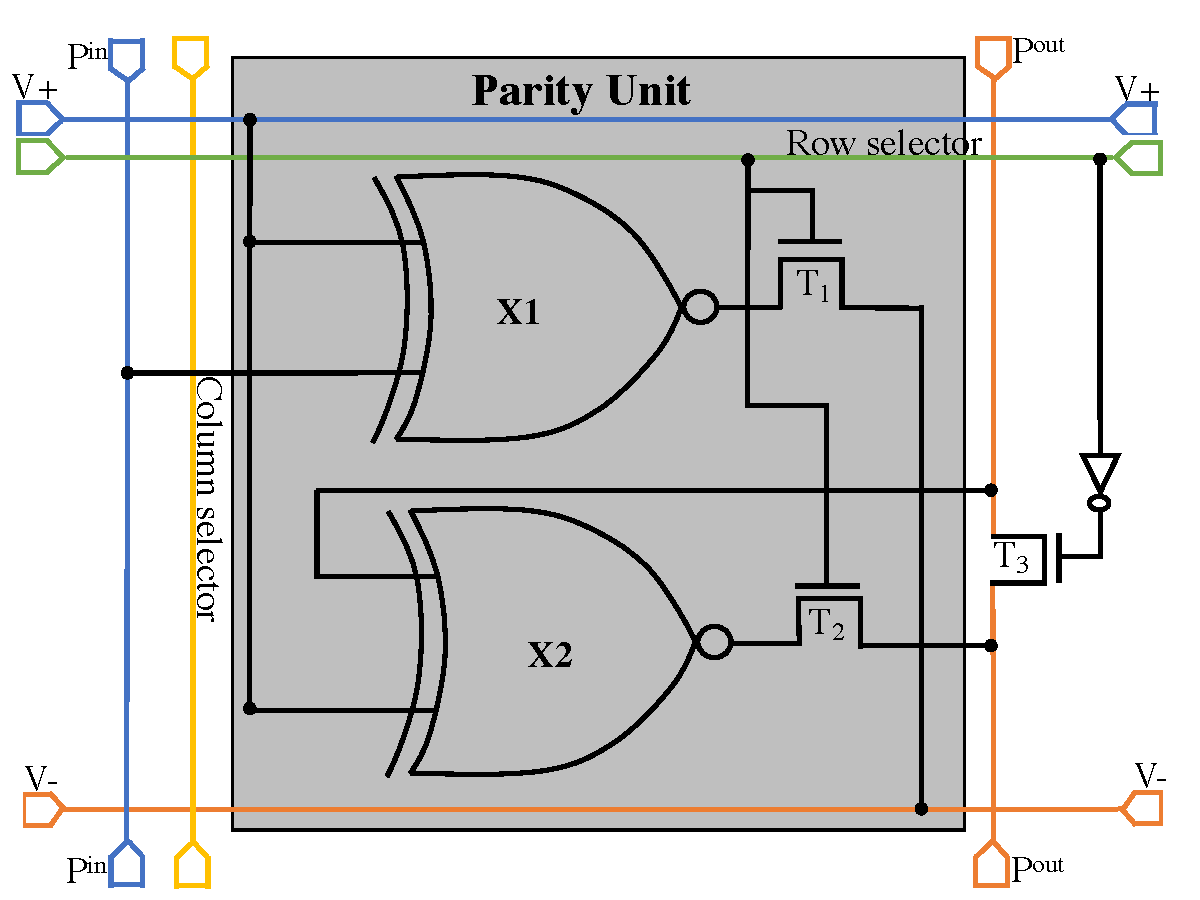
\includegraphics[width=0.5\textwidth]{FIGS/parity_unit_ldpc.pdf}}
    \caption{Schematic of parity unit. Color schemes are matched to system-level block diagram in Fig ~\ref{fig:BRIM_arch} }
    \label{fig:PU}
\end{figure}

\subsubsection{\bf Programming units}
Both the initial nodal values and the coupling resistances in parity units are programmable.
Programming of a resistor is achieved through a transistor with adjustable 
gate voltage.
% The details of the circuit design are discussed in Appendix~\ref{ ssec:circuit}. 
To the right of the parity unit array in 
Fig.~\ref{fig:BRIM_arch} is the programming array. This array consists of 
digital memory for storing the weights which drive an array of digital-to-analog 
converters (DACs).

A small amount of such DACs are sufficient to program all the parity units in a time-interleaved fashion per column. In such configuration, 
we need corresponding column selectors and pull-down logic as shown below 
the coupling units in Fig.~\ref{fig:BRIM_arch}.

\subsubsection{\bf Annealing control}\label{ssec:anneal_control}

As our system is primarily an optimizer, it can get stuck in local minima. To avoid this, two commonly used mechanisms for annealers were adopted and incorporated to allow the system to escape local optima. First, the coupling strength is globally increased over time. In this way, at the very beginning, the machine is only weakly coupled, rendering the energy landscape relatively flat. It helps the system explore the landscape in a coarse granularity. We choose an exponential annealing schedule because (a) it is a common practice, and (b) it can be conveniently achieved by discharging an appropriately-sized capacitor as the global annealing scheduler. The voltage from this capacitor is then used to control the variable gain buffer in each node to achieve the change in coupling strength.

Second, we adopt a similar strategy as that used in simulated annealing. In Simulated annealing, the spins are flipped based on a probability decided by the differences in the energy. Doing the same thing in hardware is a complex process. To simplify the process, we use a "spin fix"; we randomly choose a node and briefly clip it to one of the supply rails. The nodal spin either maintains its current state or swaps to the opposite state. The probability/frequency of spin fixes is determined based on temperature. The temperature follows the same exponential annealing schedule discussed above. In other words, the frequency of spin fixes decays exponentially over time.



\subsection{Theoretical analysis}

We can theoretically define the evolution of above described LDPC decoder using equation~\ref{eqn:rim_node_simplifed}. It shows how the voltage of a capacitor representing each node change over time. $J_{ij}$ represents the effective conductance of the coupling with the parity equations. $B_i$ represents the bias current representing the bias term in the equation~\ref{eq::LDPC_ising} and  $g_{\!_{ZIV}}(v_{i})$ represents the current due to $ZIV$ diode.

\begin{equation}\label{eqn:rim_node_simplifed}
\begin{split}
    \dv{v_i}{t} = \frac{1}{C}(I_{in} - I_{ZIV}) =  \frac{1}{C} \left[ \sum_{\mathclap{j}} J_{ij} P_{j\backslash i} + B_i - g_{\!_{ZIV}}(v_{i}) \right]
\end{split}
\end{equation}

With this equation, we can provide the same Lyapunov stability analysis as shown in the following paper~\cite{afoakwa.hpca21} to prove our ability for optimum-seeking.
\end{comment}

\begin{comment}
\todo{The commented section was not checked in editing -Andrew}

\subsection{Theoretical analysis} \label{ssec:theory}

\todo{Need to be modified}
We present same  Lyapunov stability analysis
of our LDPC decoder to show its ability for optimum-seeking as shown in the following paper~\cite{afoakwa.hpca21}.
Fig.~\ref{fig:brim} shows a simplified node $i$ in LDPC decoder where other nodes are 
coupled into $i$ from the right.
Writing the current equation, we get Eq.~\ref{eqn:rim_node_simplifed}, where $J_{ij}$ is the 
effective conductance of the coupling taking into account the polarity of
the coupling:
\begin{equation}\label{eqn:rim_node_simplifed}
\begin{split}
    \dv{v_i}{t} = \frac{1}{C}(I_{in} - I_{ZIV}) =  \frac{1}{C} \left[ \sum_{\mathclap{j}} J_{ij} P_{j\backslash i} - g_{\!_{ZIV}}(v_{i}) \right]
\end{split}
\end{equation}

LDPC decoder is a continuous time system where the state is summarized by
$v(t)=[v_1(t), v_2(t), ...\,, v_N(t)]^T$. (For brevity, in the following, $v_i(t)$
will be abbreviated as $v_i$.) Recall that in Lyapunov analysis, if a function
$H(v)$ can be found such that $\dv{H(v)}{t} = 0$ at point $v^e$
and $\dv{H(v)}{t} < 0$ in the region around $v^e$, then $v^e$ is the
equilibrium point~\cite{nonlinear_system_analysis}. In our case, this point is the solution to the equation set
$\dv{v_i}{t} = 0;\ i=1..N$.
\donotshow{\footnote{For those unfamiliar with the analysis, here is a roughly
explanation: if the condition $\dv{H(v)}{t} \leq 0$ is satisfied in a region
$v \in W$, that means once the system enters region $W$ at time $t_0$,
function $H(v(t))$ can only decrease or maintain its value (because its time
derivative is non-positive), thus a future state then clearly $H(v)$ can not
increase for a dynamical system can be identified, the system can be shown to
be stable at points where the function reaches minimum.}}
In other words, once the system enters a region, it will inevitably evolve
towards lowering $H(v)$ (because its time derivative is negative) until
it reaches the equilibrium point $v^e$.

To ensure $\dv{H(v)}{t}$ is non-positive, we can construct
it to be in a negative square form. This can be achieved 
by imposing the following construction rule.
\begin{equation}
\label{eqn:rule}
\pdv{H(v)}{v_i}=-\alpha\dv{v_i}{t}; \ \alpha>0
\end{equation} 

Following the chain rule, it is not difficult to see that:
\begin{equation}
\label{eqn:H_partials}
\dv{H(v)}{t} =\sum_{\mathclap{i}}\left(\pdv{H(v)}{v_i}\dv{v_i}{t} \right)
=-\alpha\sum_{\mathclap{i}}\left(\dv{v_i}{t}\right)^2
\end{equation}

One choice of a Lyapunov function satisfying the conditions in Eq.
\ref{eqn:rule} is shown in Eq.~\ref{eqn:Lyap_RIM}, where $G(v_i)$ is obtained
from $g_{\!_{ZIV}}(v_i)$ by integration over $v_i$. 
\begin{equation}
\label{eqn:Lyap_RIM}
H(v)= \frac{\alpha}{C}\Big(-\sum_{\mathclap{i}} \sum_{\mathclap{j}} J_{ij} P_{j\backslash i} v_i + \sum_i G(v_i)\Big)
\end{equation}
It is important to
notice that the ``Z" shape of $g_{\!_{ZIV}}(v)$ will give $P(v)$ a double-well
profile (as shown in Fig.~\ref{fig:brim}-right) with two stable equilibrium points at voltages corresponding to two
non-trivial zero-crossings of the IV curve (\eg $v_i= \pm 1V $) and a saddle
point at $v_i=0V$. Given the double-well profile of $P(v)$, the state of a
stable solution will consist of voltages at (or at least very close to) 
these equilibria (\eg $\pm 1V$).
Thus, the second term of Eq.~\ref{eqn:Lyap_RIM} will be (close to) a constant. 
Consequently, minimizing $H(v)$ is equal to minimizing the first term $-\sum_{i<j}J_{ij}v_iP_{j\backslash i}$, which is the Ising formula.

% \begin{figure}[htp]\centering
%     
\includegraphics[width=0.4\textwidth]{double_well.pdf}
%     \caption{\fixme{double well of the -P(v)}}
%     \label{fig:double_well}
% \end{figure}

%Since function $H(v)$ satisfies the conditions in Eq.
%\ref{eqn:H_partials} for all $i's$ representing a sufficient condition
%for $\frac{dH(v)}{dt}=-\sum_{i}\frac{\partial H(v_i)}{\partial
%v_i}\frac{dv_i}{dt}\leq0$, the system is stable in the Lyapunov sense and it
%is guaranteed to converge to a minimum of $H(v)$.

Note that this analysis does not guarantee that the system will converge to a
\emph{global} minimum as it depends on the energy landscape and initial 
conditions. This is similar to other annealers: None 
has strong guarantees for reaching ground state in a typical usage scenario
(as opposed to ideal conditions) or in an efficient manner. For example, it
is shown that simulated annealing can reach ground state in a system with
a finite phase space. However, the time it takes to do so may be longer than
enumerating the space~\cite{varty2017simulated}.
\end{comment}
